% Options for packages loaded elsewhere
\PassOptionsToPackage{unicode}{hyperref}
\PassOptionsToPackage{hyphens}{url}
\documentclass[
  10pt,
]{article}
\usepackage{xcolor}
\usepackage[margin=20mm]{geometry}
\usepackage{amsmath,amssymb}
\setcounter{secnumdepth}{-\maxdimen} % remove section numbering
\usepackage{iftex}
\ifPDFTeX
  \usepackage[T1]{fontenc}
  \usepackage[utf8]{inputenc}
  \usepackage{textcomp} % provide euro and other symbols
\else % if luatex or xetex
  \usepackage{unicode-math} % this also loads fontspec
  \defaultfontfeatures{Scale=MatchLowercase}
  \defaultfontfeatures[\rmfamily]{Ligatures=TeX,Scale=1}
\fi
\usepackage{lmodern}
\ifPDFTeX\else
  % xetex/luatex font selection
\fi
% Use upquote if available, for straight quotes in verbatim environments
\IfFileExists{upquote.sty}{\usepackage{upquote}}{}
\IfFileExists{microtype.sty}{% use microtype if available
  \usepackage[]{microtype}
  \UseMicrotypeSet[protrusion]{basicmath} % disable protrusion for tt fonts
}{}
\makeatletter
\@ifundefined{KOMAClassName}{% if non-KOMA class
  \IfFileExists{parskip.sty}{%
    \usepackage{parskip}
  }{% else
    \setlength{\parindent}{0pt}
    \setlength{\parskip}{6pt plus 2pt minus 1pt}}
}{% if KOMA class
  \KOMAoptions{parskip=half}}
\makeatother
\usepackage{longtable,booktabs,array}
\usepackage{calc} % for calculating minipage widths
% Correct order of tables after \paragraph or \subparagraph
\usepackage{etoolbox}
\makeatletter
\patchcmd\longtable{\par}{\if@noskipsec\mbox{}\fi\par}{}{}
\makeatother
% Allow footnotes in longtable head/foot
\IfFileExists{footnotehyper.sty}{\usepackage{footnotehyper}}{\usepackage{footnote}}
\makesavenoteenv{longtable}
\usepackage{graphicx}
\makeatletter
\newsavebox\pandoc@box
\newcommand*\pandocbounded[1]{% scales image to fit in text height/width
  \sbox\pandoc@box{#1}%
  \Gscale@div\@tempa{\textheight}{\dimexpr\ht\pandoc@box+\dp\pandoc@box\relax}%
  \Gscale@div\@tempb{\linewidth}{\wd\pandoc@box}%
  \ifdim\@tempb\p@<\@tempa\p@\let\@tempa\@tempb\fi% select the smaller of both
  \ifdim\@tempa\p@<\p@\scalebox{\@tempa}{\usebox\pandoc@box}%
  \else\usebox{\pandoc@box}%
  \fi%
}
% Set default figure placement to htbp
\def\fps@figure{htbp}
\makeatother
\setlength{\emergencystretch}{3em} % prevent overfull lines
\providecommand{\tightlist}{%
  \setlength{\itemsep}{0pt}\setlength{\parskip}{0pt}}
\usepackage{fontspec}
\usepackage{xeCJK}
\setCJKmainfont{Microsoft YaHei}
\setmainfont{TeX Gyre Termes}
\usepackage{tikz,pgfplots}
\pgfplotsset{compat=1.18}
\usepackage{float}
\let\origfigure\figure
\let\endorigfigure\endfigure
\renewenvironment{figure}[1][]{\origfigure[H]}{\endorigfigure}
\usepackage{graphicx}
\setlength{\emergencystretch}{3em}
\usepackage{fancyhdr}
\pagestyle{fancy}
\fancyhf{}
\fancyfoot[C]{\thepage}
\renewcommand{\headrulewidth}{0pt}
\usepackage{bookmark}
\IfFileExists{xurl.sty}{\usepackage{xurl}}{} % add URL line breaks if available
\urlstyle{same}
\hypersetup{
  hidelinks,
  pdfcreator={LaTeX via pandoc}}

\author{}
\date{}

\begin{document}

\section{Stage nine: alignment, score thresholds and nucleus-center
detection}\label{stage-nine-alignment-score-thresholds-and-nucleus-center-detection}

November 18--20, 2026. The main finding is that alignment dependence and
low prediction scores are distinct failure modes. The all-layer detector
benefits most from combining positions across alignments; the
translation-trained detector locates many nuclei at scores below the
threshold previously used. A fixed diagnostic of preserved predictions
now separates these cases object by object.

This report covers the useful sequence of experiments, rather than only
the newest result: the earlier translation-trained detector (P15),
full-depth adaptation (P22), intermediate-map and interpolation
diagnosis (D32/D33), position readout (P34), sixteen aligned score maps
(P35), threshold and point consensus (P36), and the new saved-point
diagnostic (D37). D32/D33 supply context; P34--D37 are the current
stage.

Eight P36 scientific computations completed. Seven array tasks finished
normally; P15 translation-trained seed 19 failed during preservation
after computation, and preservation-only job 55895127 completed
successfully. Eight collection receipts passed; 242 collected files
matched their preserved hashes. All paired decisions and the published
P36 analysis were independently reproduced. D37 replayed every original,
selected-threshold and consensus count per image before partitioning
misses. The partial P34 all-layer seed-1 run remains preserved with no
completed evaluation.

\newpage

\section{Detectors, images and
interpretation}\label{detectors-images-and-interpretation}

All eight detectors use their last checkpoint after 130 training epochs.
P22 C updates the last twelve encoder layers, and P22 M updates all
twenty-four. P15 C is its own last-twelve control; P15 J was trained
with integer translation up to sixteen pixels per axis. Each recipe has
seeds 19 and 1. P15 and P22 controls are different training runs and are
compared with their own paired experiments.

All measurements use the established fold-1 training/development
division: 2,134 training images and 522 development images. P36 samples
240 training images by a fixed hash of their number; these contain 5,581
annotated nuclei. The development set has 12,250 nuclei and 145 interior
Dead nuclei. The latter includes apoptotic and necrotic nuclei. Central
analyses use 7,014 development nuclei at least 24 pixels from all
borders, visible at all sixteen alignments.

A point is matched within three pixels of its annotated center using
maximum-cardinality one-to-one assignment. The sixteen alignments move
each axis by −8, −4, 0 or 4 pixels. White and mirrored fills are
recorded separately. Predictions are returned to original coordinates.
Threshold and consensus parameters were selected on shifted training
images and written before development images were read; the trained
alignment was excluded from selection.

Precision is the share of predicted points matched to an annotation;
recall is the share of annotated nuclei matched. F1 is their harmonic
mean. These are center-detection measurements from CPU single precision.
The original BF16 records are retained separately; this stage uses the
single-precision paired controls. Repeated alignments observe the same
nucleus and are not independent samples. Three-fold instance
segmentation and official PanNuke metrics belong to a later method
evaluation.

\newpage

\section{Position readout and averaged score maps: what the earlier
experiments
established}\label{position-readout-and-averaged-score-maps-what-the-earlier-experiments-established}

P34 trained a 73,986-parameter position readout while keeping each
detector frozen. Three tasks completed; the fourth stopped at the second
readout's first-epoch time guard (1,400.3 seconds against 1,300). No
final two-seed all-layer result is available.

The readout places the center within three pixels for 99.4\%--99.8\% of
nuclei on the 48 selected training images, versus 70.6\%--80.6\% on
development images depending on the readout and detector. Moving and
merging predicted points adds 158, 172 and 172 matches for the three
detectors and loses 173, 182 and 158. Its position error is therefore
large enough to undo almost as many valid matches as it creates.
Training the readout with translation improves its shifted-image
localization, but the final detection changes remain small.

The frozen detector itself matches 96.0\%--98.2\% on these training
images; moving the same images by (5,3) pixels reduces matching to
56.1\%--64.6\%. P35 extends this observation to sixteen alignments.
Among central training nuclei, the original alignment matches
97.4\%--99.2\%, compared with 67.1\%--72.6\% at the other fifteen. The
central development rates at the original and other alignments remain
close, at roughly 61\%--68\%.

P35 also finds that 86\%--89\% of central development nuclei are matched
at some alignment, while 51\%--61\% are matched at only some of the
sixteen. Directly averaging narrow, displaced score peaks at threshold
0.5 matches only 9\%--15\% of all development nuclei at 95\%--96\%
precision. The observed peak displacement and score reduction motivate
combining point positions and studying thresholds separately.

\begin{center}
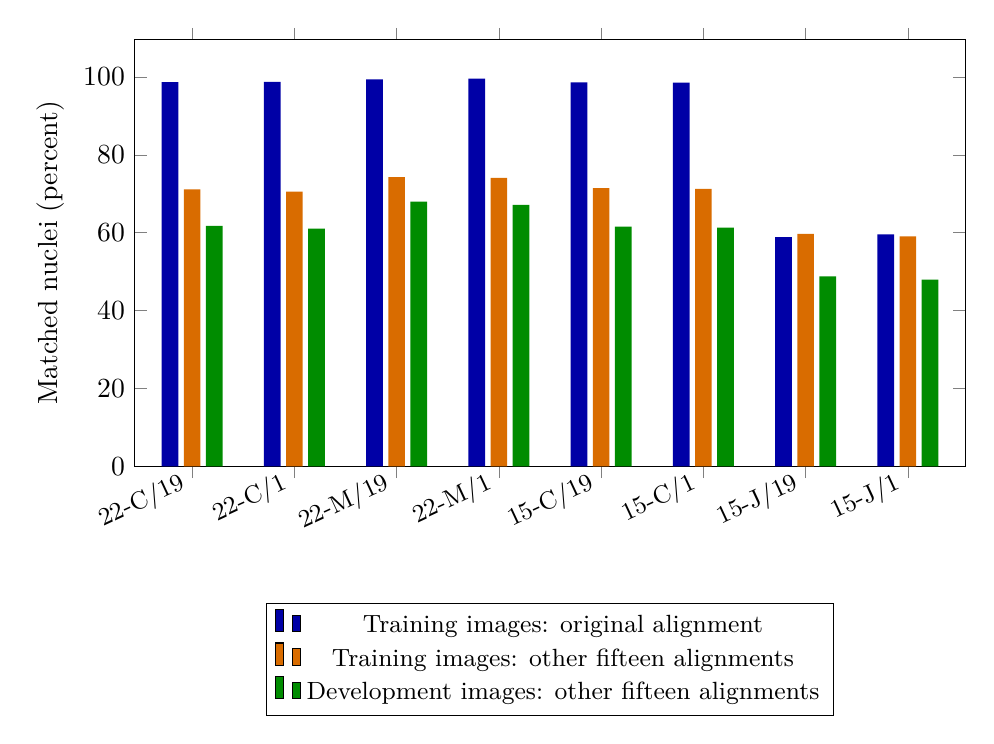
\begin{tikzpicture}
\begin{axis}[width=\linewidth,height=7cm,ymin=0,xtick={0,1,2,3,4,5,6,7},xticklabels={22-C/19,22-C/1,22-M/19,22-M/1,15-C/19,15-C/1,15-J/19,15-J/1},x tick label style={font=\small,rotate=25,anchor=east},ylabel={Matched nuclei (percent)},legend style={at={(0.5,-0.32)},anchor=north,legend columns=1,font=\small},enlarge x limits=0.08,ybar,bar width=6pt]
\addplot[fill=blue!65!black,draw=none] coordinates {(0,98.654846) (1,98.715989) (2,99.388566) (3,99.602568) (4,98.593702) (5,98.563131) (6,58.850504) (7,59.584225)};
\addplot[fill=orange!85!black,draw=none] coordinates {(0,71.150515) (1,70.537043) (2,74.285132) (3,74.103740) (4,71.478651) (5,71.282992) (6,59.702436) (7,59.082849)};
\addplot[fill=green!55!black,draw=none] coordinates {(0,61.777398) (1,61.091151) (2,67.968824) (3,67.191332) (4,61.573044) (5,61.304059) (6,48.817603) (7,47.957418)};
\legend{Training images: original alignment,Training images: other fifteen alignments,Development images: other fifteen alignments}
\end{axis}
\end{tikzpicture}
\end{center}

P36 repeats the alignment comparison on 240 training images. Labels
22-C, 22-M, 15-C and 15-J denote the four defined recipes; the suffix is
the seed. Bars use central nuclei and mirrored fill.

\newpage

\section{Threshold selection recovers low-score
nuclei}\label{threshold-selection-recovers-low-score-nuclei}

The selected threshold is 0.3 for all last-twelve controls and all-layer
seed 19, 0.4 for all-layer seed 1, and 0.2 for both translation-trained
detectors. These values were selected on shifted training images by F1
over all annotated nuclei, pooling both fills.

The translation-trained detector is the clear change. At threshold 0.5
it matches 4,771/4,600 development nuclei with 86.57\%/86.38\% precision
and 44/44 interior Dead matches. At the training-selected threshold 0.2
it matches 8,463/8,542 nuclei with 66.04\%/66.50\% precision and 101/99
interior Dead matches. The matched count increases by 3,692/3,942 with
no lost original match in the saved-record replay. This gain comes with
many new unmatched predictions.

For the all-layer detector, selected thresholds add 293/145 matches and
two interior Dead matches in each seed. Their F1 increases by only
0.0034/0.0015. Translation-trained and control models therefore require
different score interpretation; the earlier P15 verdict at fixed
threshold 0.5 remains part of that original recipe's history. The new
decoder answers a different, explicitly training-selected question.

The translation-trained model's threshold-selected training F1 is about
0.795/0.796, while development F1 is 0.675/0.681. Translation reduces
the special advantage of the original alignment; a substantial
training-to-development gap still remains.

\begin{longtable}[]{@{}lrrrrrr@{}}
\toprule\noalign{}
Recipe / seed & Cutoff & Matched / points & Dead / 145 & Recall &
Precision & F1 \\
\midrule\noalign{}
\endhead
\bottomrule\noalign{}
\endlastfoot
22-C/19 & 0.3 & 7,622 / 11,430 & 76 & 62.22\% & 66.68\% & 0.6438 \\
22-C/1 & 0.3 & 7,606 / 11,324 & 69 & 62.09\% & 67.17\% & 0.6453 \\
22-M/19 & 0.3 & 8,272 / 11,677 & 87 & 67.53\% & 70.84\% & 0.6914 \\
22-M/1 & 0.4 & 8,078 / 11,173 & 86 & 65.94\% & 72.30\% & 0.6897 \\
15-C/19 & 0.3 & 7,569 / 11,463 & 77 & 61.79\% & 66.03\% & 0.6384 \\
15-C/1 & 0.3 & 7,707 / 11,454 & 66 & 62.91\% & 67.29\% & 0.6503 \\
15-J/19 & 0.2 & 8,463 / 12,814 & 101 & 69.09\% & 66.04\% & 0.6753 \\
15-J/1 & 0.2 & 8,542 / 12,846 & 99 & 69.73\% & 66.50\% & 0.6807 \\
\end{longtable}

\newpage

\section{Combining point positions: useful gains and the remaining
tradeoff}\label{combining-point-positions-useful-gains-and-the-remaining-tradeoff}

Consensus groups points scoring at least 0.5 from the fifteen shifted
alignments around a highest-scoring point, then averages their
positions. Every detector selects radius four pixels. Last-twelve
controls select four or six contributing alignments; the all-layer
detectors select five or six; both translation-trained detectors select
one. The number is relative to alignments valid at that position.

All-layer seed 19 gains 1,163 matches and loses 871, a net 292; seed 1
gains 1,096 and loses 825, a net 271. Interior Dead matches change from
85 to 99 and 84 to 89. Precision changes from 72.90\% to 73.63\% and
73.43\% to 72.29\%. The primary two-seed criteria remain unmet: the
precision floor is 75\%, and seed 1's Dead gain is 5/145 with a paired
interval spanning zero (−0.0204 to 0.1000).

The translation-trained consensus raises recall from 38.95\%/37.55\% to
52.86\%/52.24\%, while retaining precision above 80\%. It gains
1,826/1,906 nuclei and loses 122/107. Its one-alignment rule reflects
less complementary variation among its predictions, compared with
detectors trained at one alignment. The threshold-selected decoder has
much higher recall; the consensus still discards all phase points
scoring below 0.5.

\begin{longtable}[]{@{}lrrrrrr@{}}
\toprule\noalign{}
Recipe / seed & Cutoff & Matched / points & Dead / 145 & Recall &
Precision & F1 \\
\midrule\noalign{}
\endhead
\bottomrule\noalign{}
\endlastfoot
22-C/19 & 0.5 & 7,671 / 11,050 & 84 & 62.62\% & 69.42\% & 0.6585 \\
22-C/1 & 0.5 & 7,917 / 11,543 & 94 & 64.63\% & 68.59\% & 0.6655 \\
22-M/19 & 0.5 & 8,271 / 11,233 & 99 & 67.52\% & 73.63\% & 0.7044 \\
22-M/1 & 0.5 & 8,204 / 11,348 & 89 & 66.97\% & 72.29\% & 0.6953 \\
15-C/19 & 0.5 & 7,628 / 10,963 & 80 & 62.27\% & 69.58\% & 0.6572 \\
15-C/1 & 0.5 & 7,681 / 10,957 & 81 & 62.70\% & 70.10\% & 0.6620 \\
15-J/19 & 0.5 & 6,475 / 8,006 & 71 & 52.86\% & 80.88\% & 0.6393 \\
15-J/1 & 0.5 & 6,399 / 7,863 & 69 & 52.24\% & 81.38\% & 0.6363 \\
\end{longtable}

\newpage

\section{Breast image 178: following individual
nuclei}\label{breast-image-178-following-individual-nuclei}

The four panels use the all-layer detector, seed 19: annotated centers,
original decoder, threshold 0.3 selected on training images, and
selected consensus. The image has 20 original matches, 21 at the lower
threshold and 24 with consensus. Cyan circles mark annotated centers;
green plus signs are matched points, red crosses are unmatched
predictions. Yellow indices identify interior Dead nuclei.

\begin{figure}
\centering
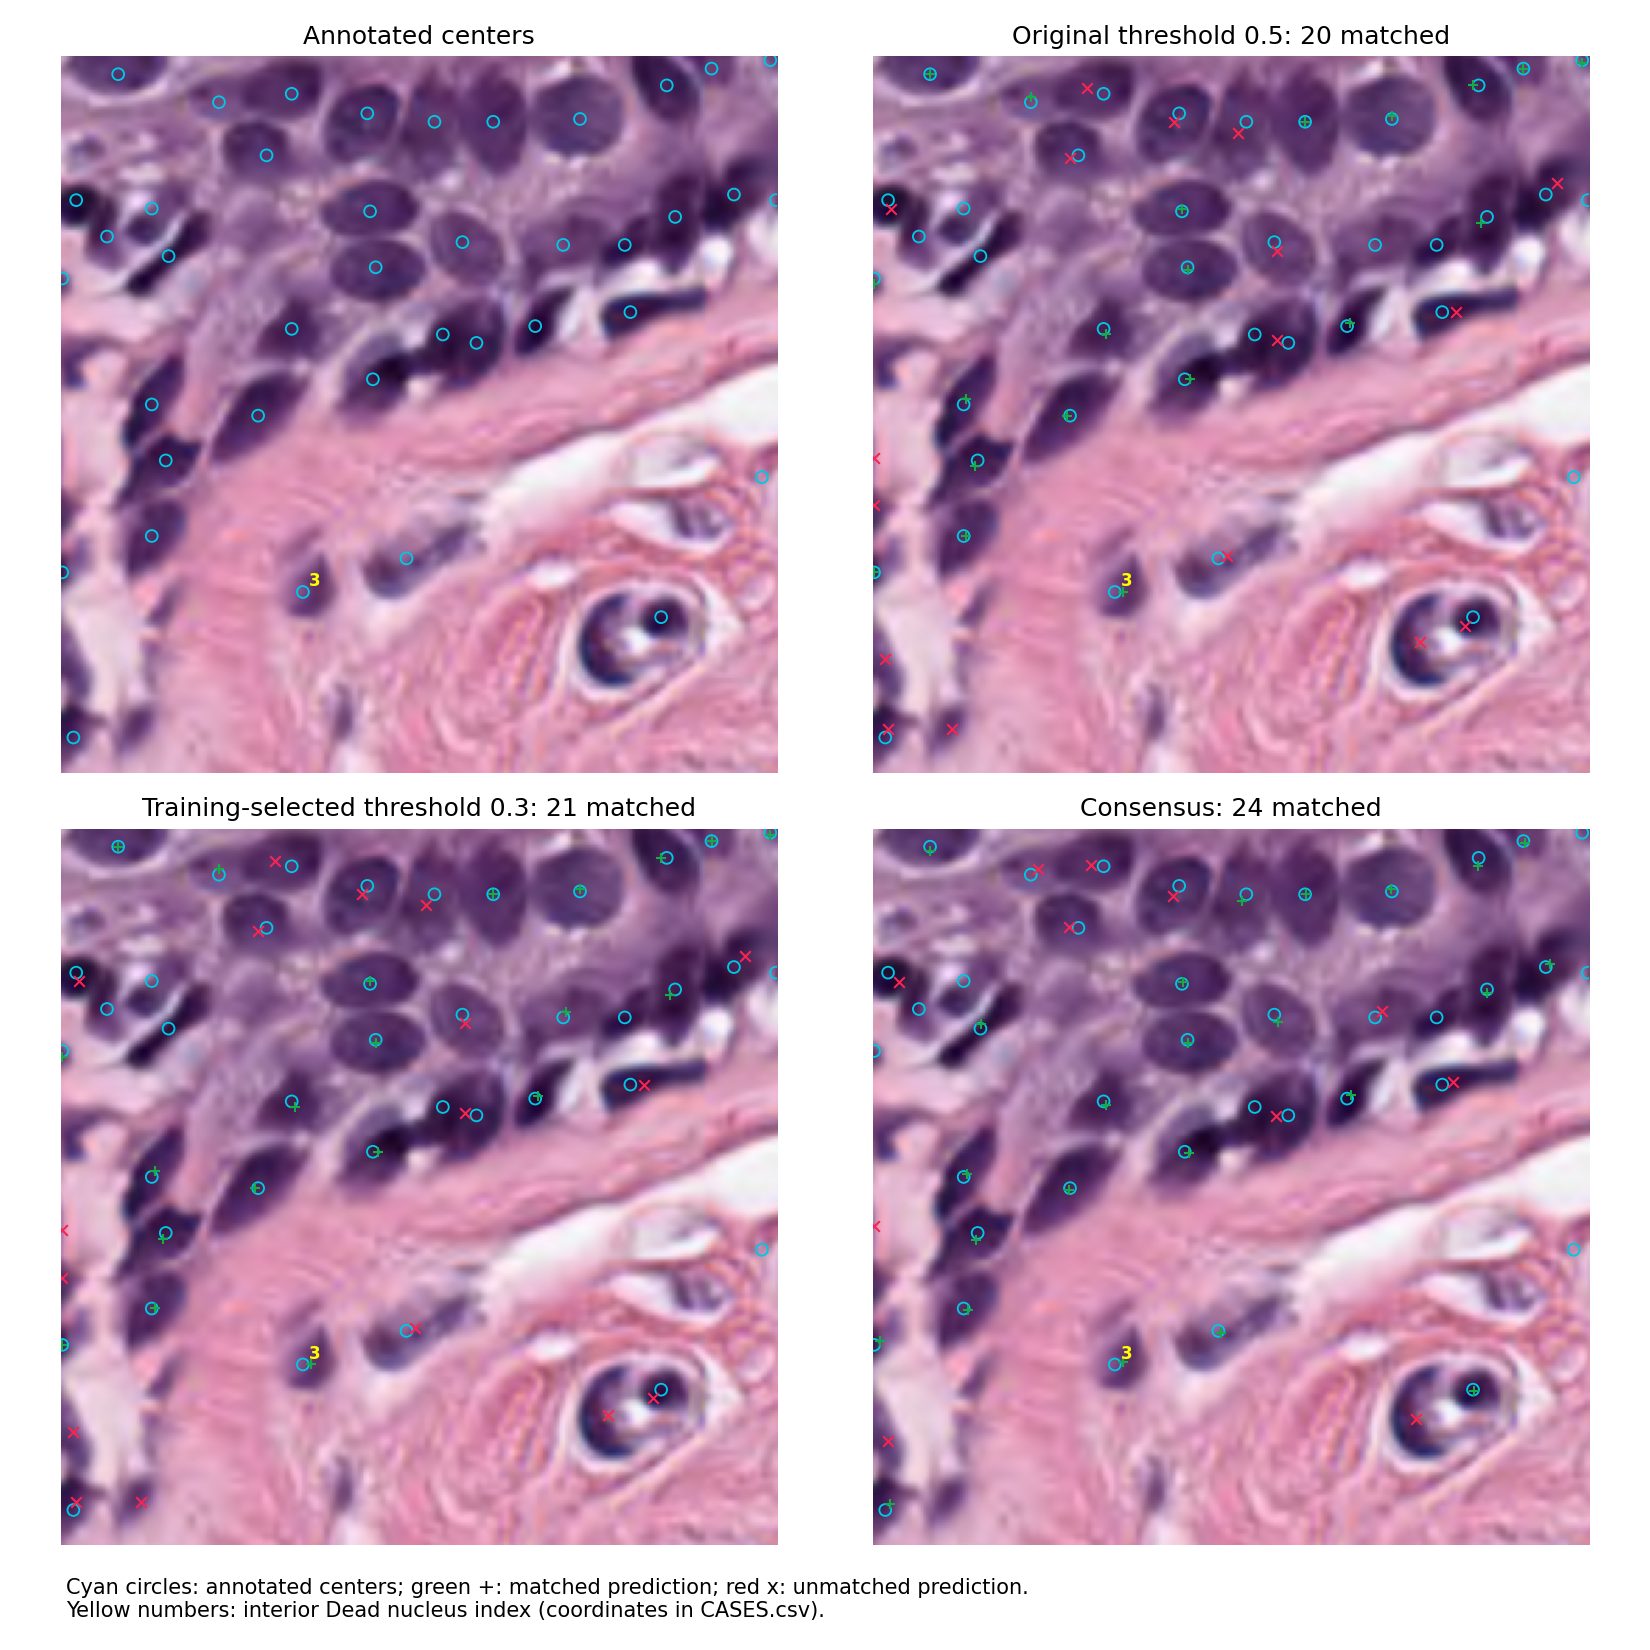
\includegraphics[width=0.9\linewidth,height=\textheight,keepaspectratio,alt={Fixed breast tissue image 178: all-layer detector, seed 19.}]{assets/P22_M_s19_development_0178.png}
\caption{Fixed breast tissue image 178: all-layer detector, seed 19.}
\end{figure}

Object 23, an epithelial nucleus at (y,x)=(71,38), has an original peak
score 0.202 within three pixels. Neither threshold 0.5 nor 0.3 retains
that peak. Four shifted alignments match it, and the consensus position
is (69.33,38.33), 1.70 pixels from the annotation. Combining shifted
positions therefore recovers this object.

Interior Dead object 3 at (191,86), area 286 pixels, is retained in all
three decoders. Its original peak score is 0.926; the consensus point is
2.97 pixels from its center, close to the three-pixel boundary. More
views can move a valid point closer to the matching boundary as well as
rescue a miss.

\newpage

\section{Colon image 1482: score loss, recovery and persistent
misses}\label{colon-image-1482-score-loss-recovery-and-persistent-misses}

This figure uses the translation-trained detector, seed 19. Matching
rises from 12 nuclei at threshold 0.5 to 26 at selected threshold 0.2;
consensus matches 18. The central strip contains many adjacent small
annotated nuclei; the full coordinates and assignments are retained.

\begin{figure}
\centering
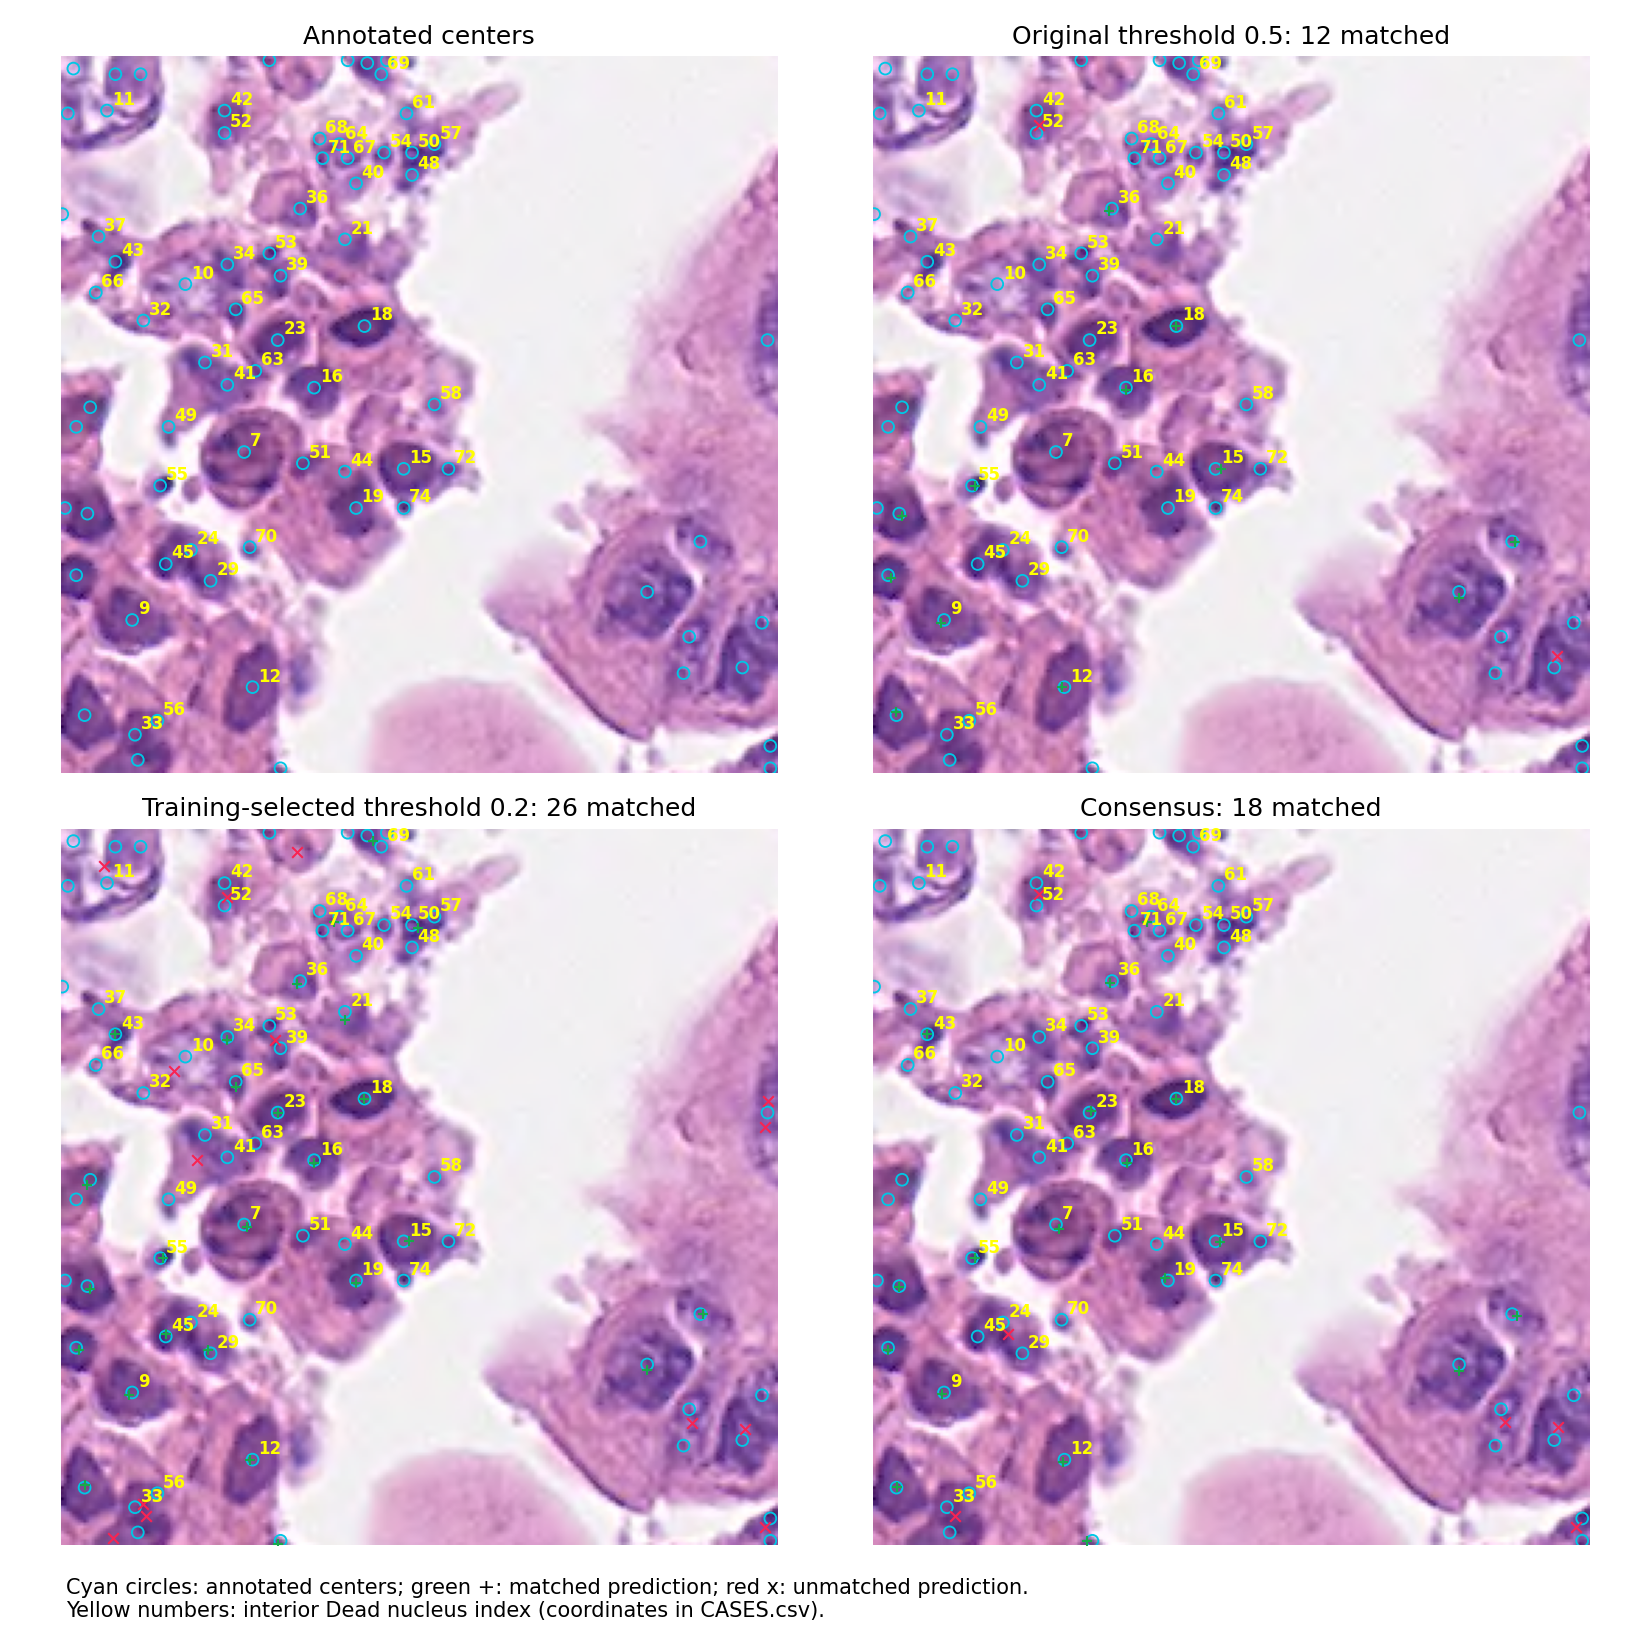
\includegraphics[width=0.9\linewidth,height=\textheight,keepaspectratio,alt={Fixed colon tissue image 1482: translation-trained detector, seed 19.}]{assets/P15_J_s19_development_1482.png}
\caption{Fixed colon tissue image 1482: translation-trained detector,
seed 19.}
\end{figure}

Dead object 7 at (141,65), area 504 pixels, has an original
center-neighborhood peak score 0.486. Threshold 0.5 removes it;
threshold 0.2 retains it. Twelve shifted alignments match it, and
consensus places a point 1.90 pixels from its annotation. Here score
threshold and alignment both account for recovery.

Dead object 51 at (145,86), area 67 pixels, remains missed by both
detectors. Neither detector has a recorded original peak at or above 0.1
within six pixels, and no alignment matches it at recording floor 0.1
within three pixels. A nearby small object, 55 at (153,35), area 57
pixels, is found by the translation-trained model (score 0.575;
consensus distance 1.11 pixels) and missed by the all-layer model. Small
area is associated with difficulty across the dataset; these two objects
show that area alone cannot explain each outcome.

\newpage

\section{D37: an exclusive partition of the remaining
misses}\label{d37-an-exclusive-partition-of-the-remaining-misses}

The new diagnostic uses preserved P36 points without another model
forward pass. In order, each nucleus is: matched originally; missed
originally but matched at another alignment at 0.5; matched only after
admitting scores down to the recording floor 0.1; near a point assigned
elsewhere; or without a recorded point within three pixels at any
alignment. Both fills and both data roles are analyzed. Lower thresholds
can alter assignment to neighboring nuclei, so the partition uses the
stated priority rather than assuming identical per-object assignments.

For all-layer seed 19, of 4,271 original misses, 2,476 (58.0\%) are
matched at another white-filled alignment at 0.5, 401 (9.4\%) only below
0.5, two involve competition, and 1,392 (32.6\%) have no recorded point
within three pixels. For translation-trained seed 19, of 7,479 original
misses, 2,104 (28.1\%) are alignment-recoverable and 4,141 (55.4\%)
require lower scores; 1,234 (16.5\%) have no recorded point within three
pixels. Seed 1 repeats the contrast.

The central-only chart below removes the border strip. The annotations
are used to ask whether a matching point exists at any alignment; this
availability statistic is separate from the selected decoder. A score
below 0.1 is not stored, and a peak farther than three pixels belongs to
the last category even when it is inside the nucleus.

\begin{center}
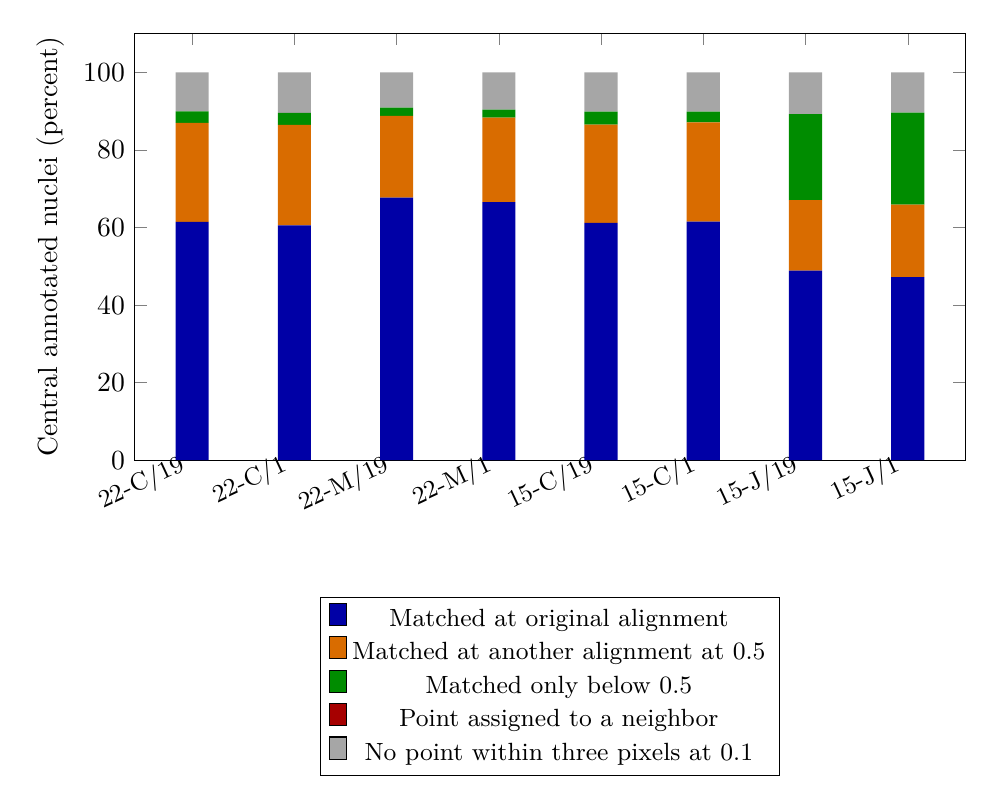
\begin{tikzpicture}
\begin{axis}[width=\linewidth,height=7cm,ymin=0,xtick={0,1,2,3,4,5,6,7},xticklabels={22-C/19,22-C/1,22-M/19,22-M/1,15-C/19,15-C/1,15-J/19,15-J/1},x tick label style={font=\small,rotate=25,anchor=east},ylabel={Central annotated nuclei (percent)},legend style={at={(0.5,-0.32)},anchor=north,legend columns=1,font=\small},enlarge x limits=0.08,ybar stacked,bar width=12pt]
\addplot[fill=blue!65!black,draw=none] coordinates {(0,61.448532) (1,60.564585) (2,67.721699) (3,66.524095) (4,61.191902) (5,61.505560) (6,48.873681) (7,47.191332)};
\addplot[fill=orange!85!black,draw=none] coordinates {(0,25.506131) (1,25.862561) (2,21.043627) (3,21.799259) (4,25.320787) (5,25.591674) (6,18.149415) (7,18.676932)};
\addplot[fill=green!55!black,draw=none] coordinates {(0,2.965498) (1,3.136584) (2,2.138580) (3,2.024522) (4,3.321928) (5,2.765897) (6,22.212717) (7,23.709723)};
\addplot[fill=red!65!black,draw=none] coordinates {(0,0.000000) (1,0.000000) (2,0.000000) (3,0.000000) (4,0.000000) (5,0.000000) (6,0.000000) (7,0.000000)};
\addplot[fill=gray!70,draw=none] coordinates {(0,10.079840) (1,10.436270) (2,9.096094) (3,9.652124) (4,10.165384) (5,10.136869) (6,10.764186) (7,10.422013)};
\legend{Matched at original alignment,Matched at another alignment at 0.5,Matched only below 0.5,Point assigned to a neighbor,No point within three pixels at 0.1}
\end{axis}
\end{tikzpicture}
\end{center}

Exclusive states for 7,014 central development nuclei; white fill. Full
all-nucleus counts are below.

\begin{longtable}[]{@{}
  >{\raggedright\arraybackslash}p{(\linewidth - 10\tabcolsep) * \real{0.1304}}
  >{\raggedleft\arraybackslash}p{(\linewidth - 10\tabcolsep) * \real{0.1739}}
  >{\raggedleft\arraybackslash}p{(\linewidth - 10\tabcolsep) * \real{0.1739}}
  >{\raggedleft\arraybackslash}p{(\linewidth - 10\tabcolsep) * \real{0.1739}}
  >{\raggedleft\arraybackslash}p{(\linewidth - 10\tabcolsep) * \real{0.1739}}
  >{\raggedleft\arraybackslash}p{(\linewidth - 10\tabcolsep) * \real{0.1739}}@{}}
\toprule\noalign{}
\begin{minipage}[b]{\linewidth}\raggedright
Recipe / seed
\end{minipage} & \begin{minipage}[b]{\linewidth}\raggedleft
Original
\end{minipage} & \begin{minipage}[b]{\linewidth}\raggedleft
Other alignment
\end{minipage} & \begin{minipage}[b]{\linewidth}\raggedleft
Low score
\end{minipage} & \begin{minipage}[b]{\linewidth}\raggedleft
Competition
\end{minipage} & \begin{minipage}[b]{\linewidth}\raggedleft
No nearby point
\end{minipage} \\
\midrule\noalign{}
\endhead
\bottomrule\noalign{}
\endlastfoot
22-C/19 & 7,255 & 2,875 & 536 & 1 & 1,583 \\
22-C/1 & 7,199 & 2,893 & 521 & 1 & 1,636 \\
22-M/19 & 7,979 & 2,476 & 401 & 2 & 1,392 \\
22-M/1 & 7,933 & 2,493 & 354 & 2 & 1,468 \\
15-C/19 & 7,255 & 2,849 & 574 & 1 & 1,571 \\
15-C/1 & 7,285 & 2,894 & 498 & 1 & 1,572 \\
15-J/19 & 4,771 & 2,104 & 4,141 & 0 & 1,234 \\
15-J/1 & 4,600 & 2,178 & 4,267 & 1 & 1,204 \\
\end{longtable}

\newpage

\section{Position variation: reduced jitter, persistent shared
displacement}\label{position-variation-reduced-jitter-persistent-shared-displacement}

For isolated central nuclei with a point within six pixels in at least
two shifted alignments, P36 separates squared displacement into an
alignment-varying component and a shared component. With mirrored fill,
last-twelve detectors have about 2.04--2.10 squared pixels of variation
and 4.29--4.42 of shared displacement. All-layer detectors have
1.67/1.68 and 3.78/3.83. Translation-trained detectors have 0.62/0.62
and 3.46/3.40.

Translation training reduces the alignment-varying quantity by roughly
70\% relative to its own controls. The shared displacement remains
larger. Averaging views can reduce variation, but it cannot remove a
common offset. This explains why stable predictions need not coincide
with the annotation.

The shared estimate is the squared mean offset minus the
within-alignment sample variance divided by the number of observed
points. This is a descriptive moment decomposition of deterministic
shifts, not a causal attribution of the offset to image content or
annotation noise. It also conditions on a nearby retained point; the
translation-trained subset contains about 4,500 nuclei versus roughly
6,300 in the other models, so the cross-model comparison is not based on
identical retained objects.

\begin{center}
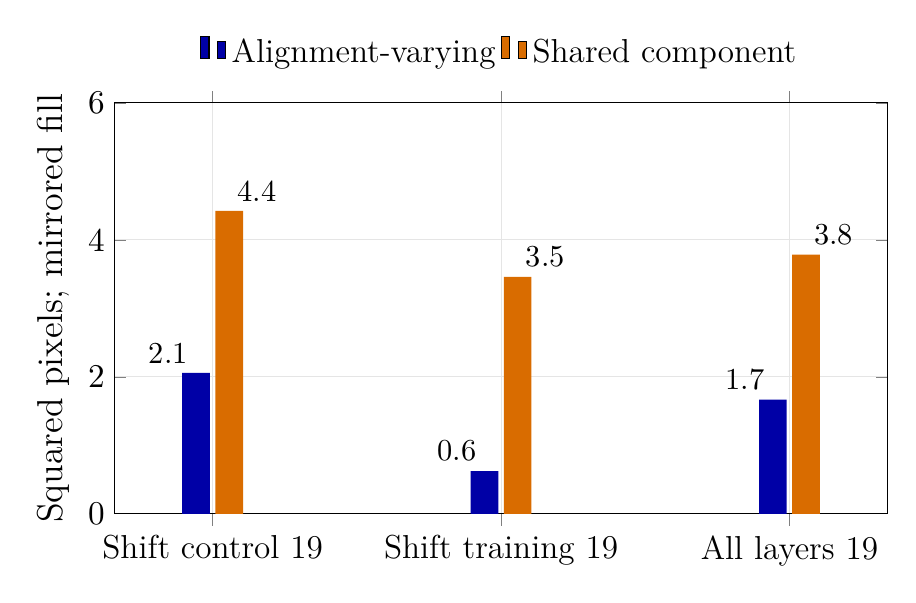
\begin{tikzpicture}
\begin{axis}[width=0.94\linewidth,height=68mm,ybar,bar width=10pt,ymin=0,ymax=6,enlarge x limits=0.17,xtick={0,1,2},xticklabels={{Shift control 19},{Shift training 19},{All layers 19}},ylabel={Squared pixels; mirrored fill},tick label style={font=\fontsize{12}{15}\selectfont},label style={font=\fontsize{13}{16}\selectfont},legend style={at={(0.5,1.06)},anchor=south,legend columns=2,draw=none,font=\fontsize{12}{15}\selectfont},grid=major,major grid style={gray!20}]
\addplot[fill=blue!65!black,draw=none,nodes near coords,nodes near coords style={font=\fontsize{11}{13}\selectfont,xshift=-10pt,/pgf/number format/fixed,/pgf/number format/precision=1}] coordinates {(0,2.05746077) (1,0.62138397) (2,1.66686793)};
\addplot[fill=orange!85!black,draw=none,nodes near coords,nodes near coords style={font=\fontsize{11}{13}\selectfont,xshift=10pt,/pgf/number format/fixed,/pgf/number format/precision=1}] coordinates {(0,4.42344983) (1,3.45747238) (2,3.78247919)};
\legend{{Alignment-varying},{Shared component}}
\end{axis}
\end{tikzpicture}

\end{center}

Development images, mirrored fill: same radius, isolation rule and
estimator for each detector. The differing retained-object subsets are
stated above.

\newpage

\section{Research decisions, reproducibility and remaining
work}\label{research-decisions-reproducibility-and-remaining-work}

The useful findings now separate three mechanisms. First, changing
alignment recovers many misses of the all-layer detector; point-position
consensus is more suitable than averaging narrow probability peaks.
Second, translation training reduces alignment variation and lowers
scores, making decoder calibration part of evaluating that recipe.
Third, about 9\%--10\% of central development nuclei still lack a
recorded point within three pixels at any alignment at 0.1 in the
all-layer and translation-trained detectors. Those objects require
further image and response analysis, with small and crowded nuclei as
concrete subgroups.

The next method experiment should couple training-selected score
calibration with positional support: P36 selects a lower threshold for
single-view decoding, but its consensus always starts at 0.5. A separate
frozen design should compare calibrated low-score consensus with the
existing P36 rule, choose parameters only on a training calibration
subset separated by image, and keep both seeds, last checkpoints and
original development criteria. No development threshold will be deployed
from the descriptive curves. No new detector training, mask expansion or
test-fold evaluation was run in this task.

D37 code and the fixed design were committed before its calculation. The
first replay omitted images with no annotated nuclei from the object
table; a focused regression and a corrected replay retain their
unmatched predictions. The failed output and log remain preserved. Final
focused validation: 33 passed, including inherited alignment behavior.
D37 replays all three decoders on 240 training and 522 development
images for all eight models. Source, hashes, full object records, eight
fixed image figures, selected case responses and build instructions are
retained.

P34's incomplete all-layer seed-1 evaluation and independent external
checkpoint archiving remain recorded tasks. A future completion of P34
requires its own explicit recovery design and resource check. GPU
allocation queries now differ from earlier accounting snapshots; this
task uses CPU saved-record analysis, preserving the budget uncertainty.
The report PDFs are compiled from the accompanying LaTeX, with
statistical charts generated by PGFPlots and actual tissue images
embedded as raster evidence.

\end{document}
